\subsection*{Sensor theory}
Sensor fusion can be observed everywhere for example living animals uses all of its senses to survive daily, e.g. a animal cannot hunt using its eyes only, it has to combine its sense of smell, eyes and hearing to hunt the pray. Sensor fusion theory is not only found in the living it can be found in cars, planes computers and so on. All this to achieve enhance the performance. In this project sensor fusion will be used to enhance the accuracy of the dinghy's position and velocity. To do so an GPS and a accelerometer will be used. \\ 
The GPS's accuracy is not uniform since it might be buildings reflections, atmospherics delays or clock bias errors. Using only information provided by a accelerometer is not sufficient either since after time the sensor will drift, using the sensor only for short time will give accurate readings.  


\subsection{Kalman Filter}
A popular filter to use when doing sensor fusion is to use a Kalman filter, (KF). The Kalman Filter is a recursive filtering method for discrete data, the algorithm was developed by an Hungarian mathematician Rudolf (Rudi) Emil Kálmán in 1960. Since everything is nonlinear in the universe, many systems cannot be seen as linear and therefore Extended Kalman, (EKF) Filter has to be applied. The EKF linearizes the system around its working points. The KF is widely used due to its efficiency when calculating the estimations. When estimating the position and velocity there will be equation which are nonlinear, hence a EKF will be applied. Where the EKF algorithm is.
\begin{align}
&\textrm{State equation} \qquad x_k=F_{k-1}x_{k-1}+v_k\\
& \textrm{Observation equation} \qquad z_k=H(x_k)+w_k
\end{align}
Where $v_k$ and $w_k$ is the process noise and measurement noise, respectively both assumed to be zero mean Gaussian noise with covariance matrices $Q_k$ and $R_k$, i.e. $v_k\in\mathcal{N}(0, Q_k)$ and $w_k\in\mathcal{N}(0, R_k)$.
\begin{align}
&\textrm{Predict state estimate:} \qquad \hat{x}_{k|k-1}=F_k\hat{x}_{k|k-1}+B_ku_k\\
&\textrm{Predict covariance matrix:}\qquad P_{k|k-1}=F_{k}P_{k-1|k-1}F^T_{k}+Q_{k}\\
\label{eq.measurement}
&\textrm{measurement residual}\qquad \tilde{y}=z_k-H_k\hat{x}_{k|k-1}\\
&\textrm{Innovation covariance}\qquad S_k=H_kP_{k|k-1}H_k^T+R_k \\
&\textrm{Near-optimal Kalman gain}\qquad K_k=P_{k|k-1}H_k^TS_k^{-1}\\
\label{eq.Update}
&\textrm{Update state estimate}\qquad \hat{x}_{k|k}=\hat{x}_{k|k-1}+K_k\tilde{y}_k\\
&\textrm{Update covariance estimate}\qquad P_{k|k}=(I-K_kH_k)P_{k|k-1}\\
&\textrm{Measurement post-fit residual} \qquad \tilde{y}_{k|k}=z_k-H_k\hat{x}_{k|k}
\end{align}
If Eq.\eqref{eq.measurement} and \eqref{eq.Update} is analyzed we see that depending on how much we believe in the observations that are observed will affect the gain matrix. Consider Fig. \ref{kalman} as a map of how the algorithm works.
\begin{figure}[H]
\centering
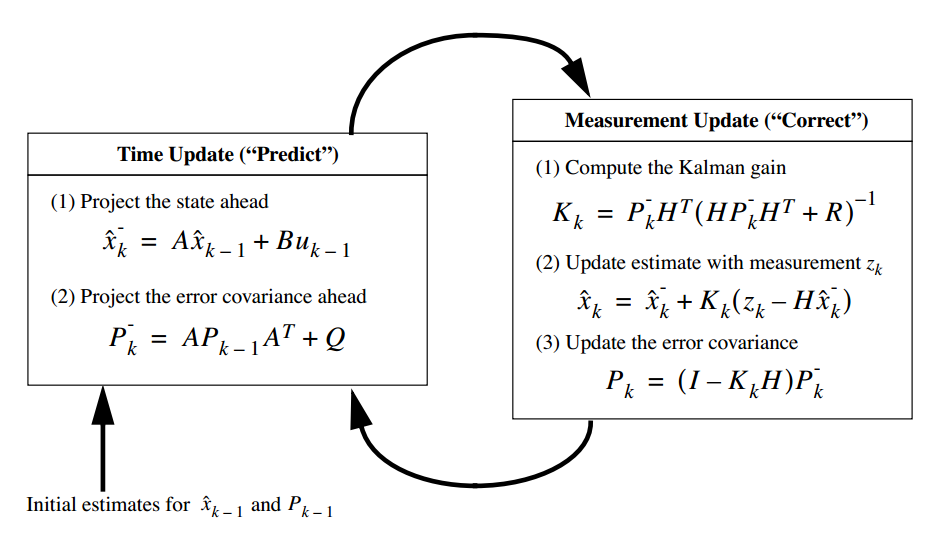
\includegraphics[width=0.8\textwidth]{kalman_algo}
\caption{}
\label{kalman}
\end{figure}

\subsection*{Integration GPS/INS}
It exist different types of integration levels most common are loosely, tightly and ultra-tightly coupled. The two last types are used when the output from the GPS receiver is its pseudo-range and carrier-range. Since the GPS receiver that is used in this project uses NMEA standard, the output will be the calculated position, velocity and heading. Then using a loosely coupled integration is preferred.\\
THE MODEL \\ 

\subsection*{Kalman Filter Model}
The states, which is chosen to observe.
\begin{align}
x=&
\begin{bmatrix}
x^{pos}\quad[m]\\
y^{pos}\quad[m]\\
v^{x}\quad[m/s]\\
v^{x}\quad[m/s]\\
\end{bmatrix}
\end{align}
$x_{pos}$ and $y_{pos}$ is the position in x and y direction, respectively, velocity, $v$, acceleration, $a$, angular position $\phi$ and angular velocity, $\dot{\phi}$. The coordinate system that is used for calculations are the \emph{WGS-84}. See Fig. \ref{bat} for a geometrical perspective.

\begin{figure}[H]
\centering
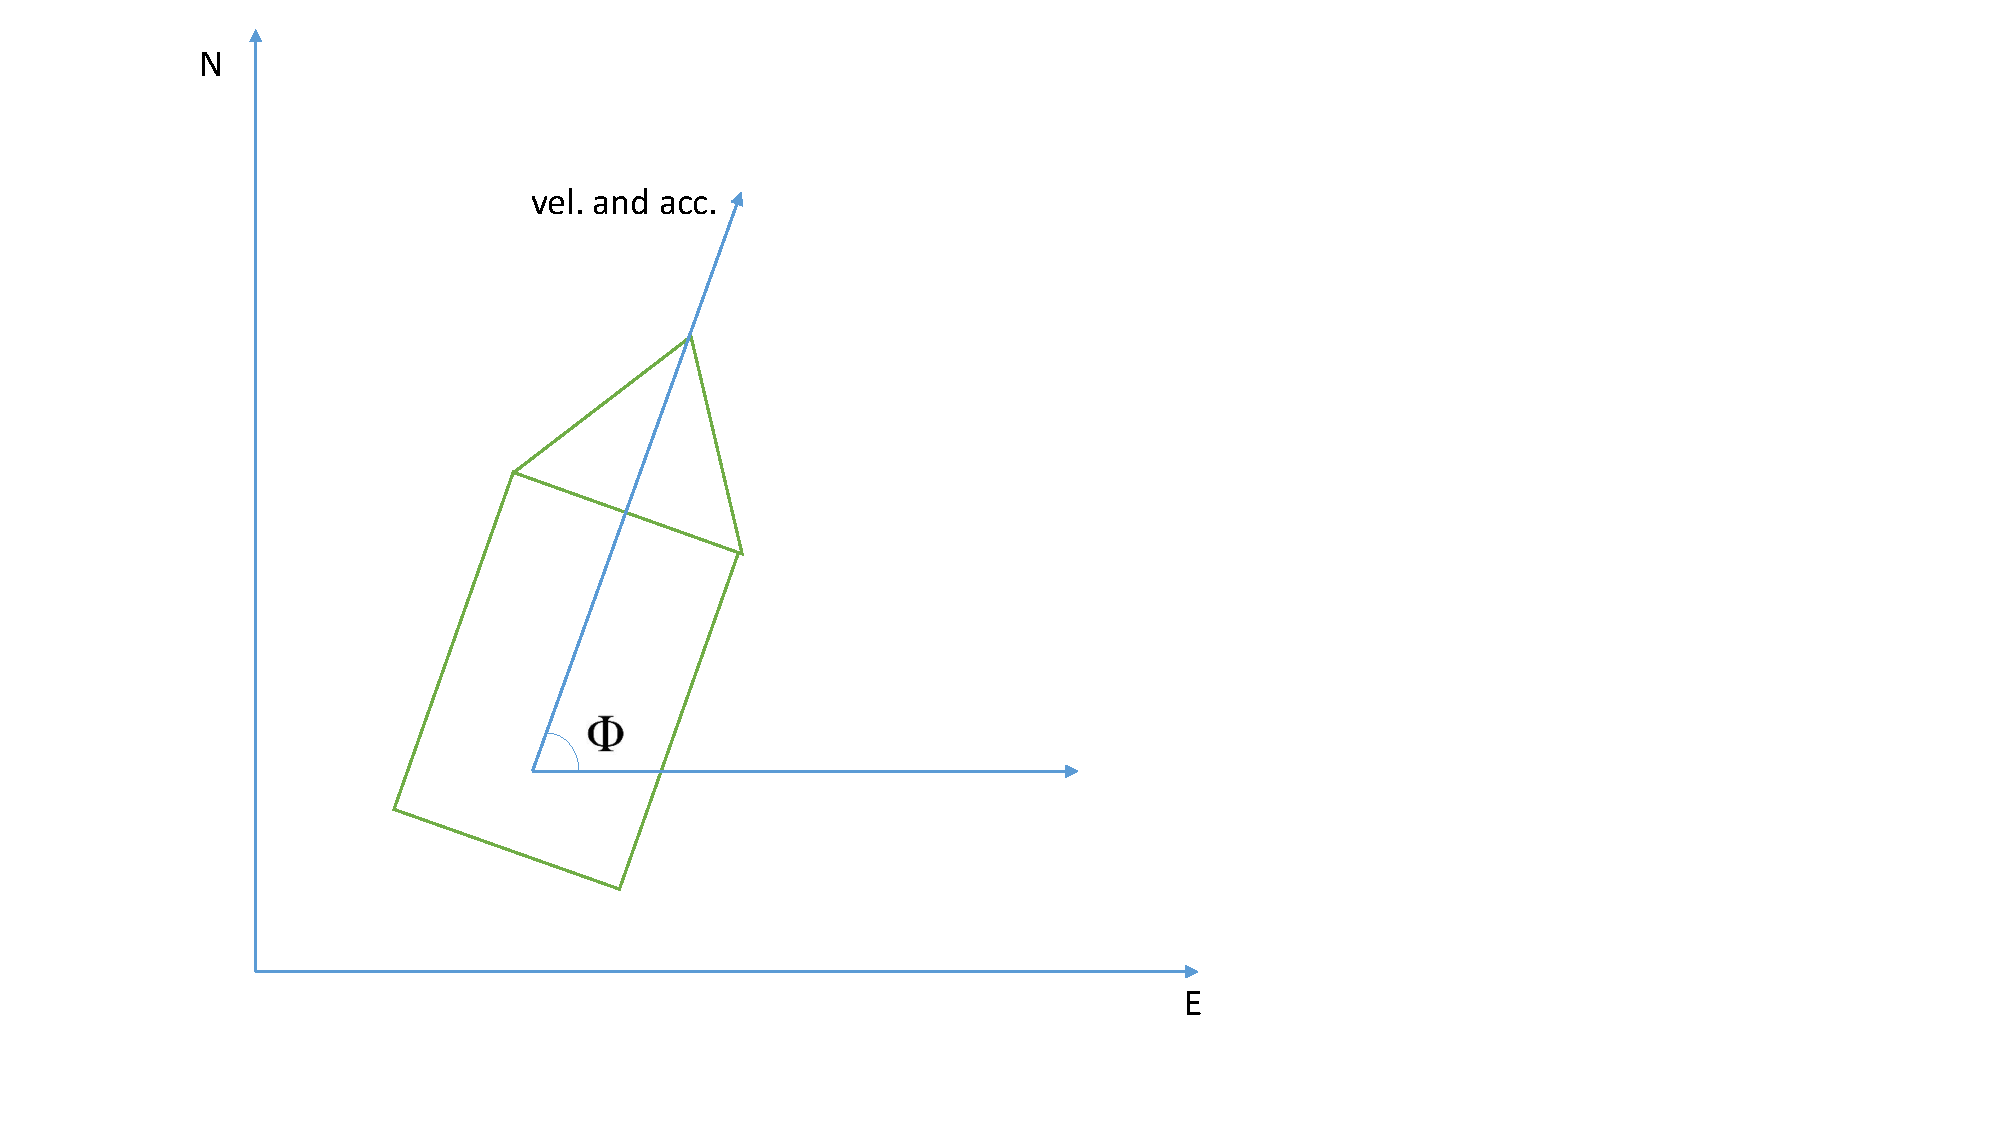
\includegraphics[width=0.8\textwidth]{b_t.pdf}
\caption{}
\label{bat}
\end{figure}

The Kalman filter calculates estimates of the true values of states recursively over time using incoming measurements and a mathematical process model, i.e. it uses $x_{k-1}$ to calculate $x_k$. Hence a mathematical model has to be derived describing the process, the GPS will provide heading position and velocity, the accelerometer will provide acceleration in $xy$-direction.\\
The model will not make an assumption that the acceleration is constant under the sampling times, this since the sampling period is $1Hz$. The process model is derived using kinematics using only $xy$-directions. Calculating the resultant velocity vector will be conducted after this since it will induce nonlinearity then extended kalman filter has to be introduced.

\begin{align}
x^{pos}_{k}&=x^{pos}_{k-1}+\Delta tv^{x}_{k-1}+\frac{1}{2}\Delta t^2a^x_{k-1}\\
y^{pos}_{k}&=y^{pos}_{k-1}+\Delta tv^{y}_{k-1}+\frac{1}{2}\Delta t^2a^y_{k-1}\\
v^{x}_{k}&=v^{x}_{k-1}+\Delta ta^x_{k-1}\\
v^{y}_{k}&=v^{y}_{k-1}+\Delta ta^y_{k-1}
\end{align}

Using the above equation the state matrix is expressed as.

\begin{align}
f=
\begin{bmatrix}
1 & 0 & \Delta t & 0 & \frac{1}{2}\Delta t^2 & 0 \\ 
0 & 1 & 0 &\Delta t & 0 & \frac{1}{2}\Delta t^2 \\ 
0 & 0 & 1 & 0 & \Delta t & 0 \\ 
0 & 0 & 0 & 1 & 0 & \Delta t \\ 
\end{bmatrix}
\qquad G=
\begin{bmatrix}
\Delta t^2 & 0\\
0 & \Delta t^2\\
\Delta t & 0\\
0 & \Delta t\\
1 & 0\\
0 & 1
\end{bmatrix}
\label{eq.F,G}
\end{align}
In The constant acceleration model the acceleration increments are assumed to have zero-mean, thus the covariance matrix is.
\begin{align}
v_k=
\begin{bmatrix}
\sigma^2_{a^x} & 0\\
0 & \sigma^2_{a^y}
\end{bmatrix}
\end{align}
Where $\sigma^2_{a^x}$ and $\sigma^2_{a^y}$ is the standard deviation squared in x and y direction respectively.
Then the covariance matrix, (the measurement noise) is derived $Q=GwG^T$.
\begin{align}
Q=
\begin{bmatrix}
\sigma^2_{a^x}\Delta t^4/4 & 0 & \sigma^2_{a^x}\Delta t^3/2 & 0 & \sigma^2_{a^x}\Delta t^2/2 & 0\\
0 & \sigma^2_{a^y}\Delta t^4/4 & 0 & \sigma^2_{a^y}\Delta t^3/2 & 0 & \sigma^2_{a^y}\Delta t^2/2\\
\sigma^2_{a^x}\Delta t^3/2 & 0 & \sigma^2_{a^x}\Delta t^2 & 0 & \sigma^2_{a^x}\Delta t & 0\\
0 & \sigma^2_{a^y}\Delta t^3/2 & 0 & \sigma^2_{a^y}\Delta t^2 & 0 & \sigma^2_{a^y}\Delta t\\
\sigma^2_{a^x}\Delta t^2/2 & 0 & \sigma^2_{a^x}\Delta t & 0 & \sigma^2_{a^x} & 0\\
0 & \sigma^2_{a^y}\Delta t^2 & 0 & \sigma^2_{a^y}\Delta t & 0 & \sigma^2_{a^y}
\end{bmatrix}
\label{eq.Q}
\end{align}

Consider \eqref{eq.F,G} and \eqref{eq.Q} we can see that the matrices are linear, this implies that a linear model approach is sufficient to use, hence a linear Kalman Filter is used. The measurement variance is user determined, more specific, it depends on the hardware and given by.

\begin{align}
R&=
\begin{bmatrix}
\sigma^2_{x^{pos}} & 0 & 0 & 0 & 0 & 0\\
0 & \sigma^2_{y^{pos}} & 0 & 0 & 0 & 0\\
0 & 0 & \sigma^2_{v^{x}} & 0 & 0 & 0\\
0 & 0 & 0 & \sigma^2_{v^{y}} & 0 & 0\\
0 & 0 & 0 & 0 & \sigma^2_{a^{x}} & 0\\
0 & 0 & 0 & 0 & 0 & \sigma^2_{a^{y}}
\end{bmatrix}
\end{align}

The output from the GPS follows\emph{WGS-84} standard this means that the GPS will provide information in global frame, i.e longitude and latitude in degrees. This has to be convert into a navigation frame




%	COVER FIGURE
%---------------------------------------------------------------------------------------https://github.com/jalishah/airborne/blob/c374b775c608de9bf8f7152aa2c79bc9e1ecec6e/ARCADE/airborne/components/core/src/model/model.c


%	ABSTRACT
%----------------------------------------------------------------------------------------



%	TABLE OF CONTENTS PAGE
%----------------------------------------------------------------------------------------
%\newpage

%\setcounter{secnumdepth}{2} % organisational level that receives a numbers
%\setcounter{tocdepth}{3}    % print table of contents for level 3
%\tableofcontents            % print the table of contents
%% levels are: 0 - chapter, 1 - section, 2 - subsection, 3 - subsubsection
%\thispagestyle{empty}
\pagebreak
%\setcounter{page}{1}







%	SECTIONS

